\documentclass[11pt, a4paper, onecolumn]{article}

\title{\textbf{Object Detection in an Image}}
\author{Bruno de Almeida Silveira}
\date{October 2019}

\usepackage{url}
\usepackage{hyperref}
\usepackage{indentfirst}

\usepackage{booktabs}
\usepackage[table,xcdraw]{xcolor}

\usepackage{adjustbox}
\usepackage{lipsum}
\usepackage{caption}

\usepackage{amsmath}

\usepackage{graphicx}

\usepackage{xurl}

\usepackage{titling}
\usepackage{blindtext}

\usepackage{subfig}

\usepackage{appendix}
\usepackage{etoolbox}
\BeforeBeginEnvironment{appendices}{\clearpage}

\graphicspath{ {./images/} }
\begin{document}

\begin{titlingpage}
	\maketitle
	\begin{abstract}
		Here comes an abstract...
	\end{abstract}
\end{titlingpage}

\section{Definition}
\subsection{Project Overview}
The main challenge in this project is to create a model that identifies many objects in an image. This challenge involves two main tasks. The former identifies in an image where it is the position of an object that could be classified, and around it, we are going to draw a bounding box. The latter classifies those bounding boxes correctly, labeling a chair as a chair, a table as a table, and a human hand as a human hand.

\begin{figure}[ht]
	\centering
	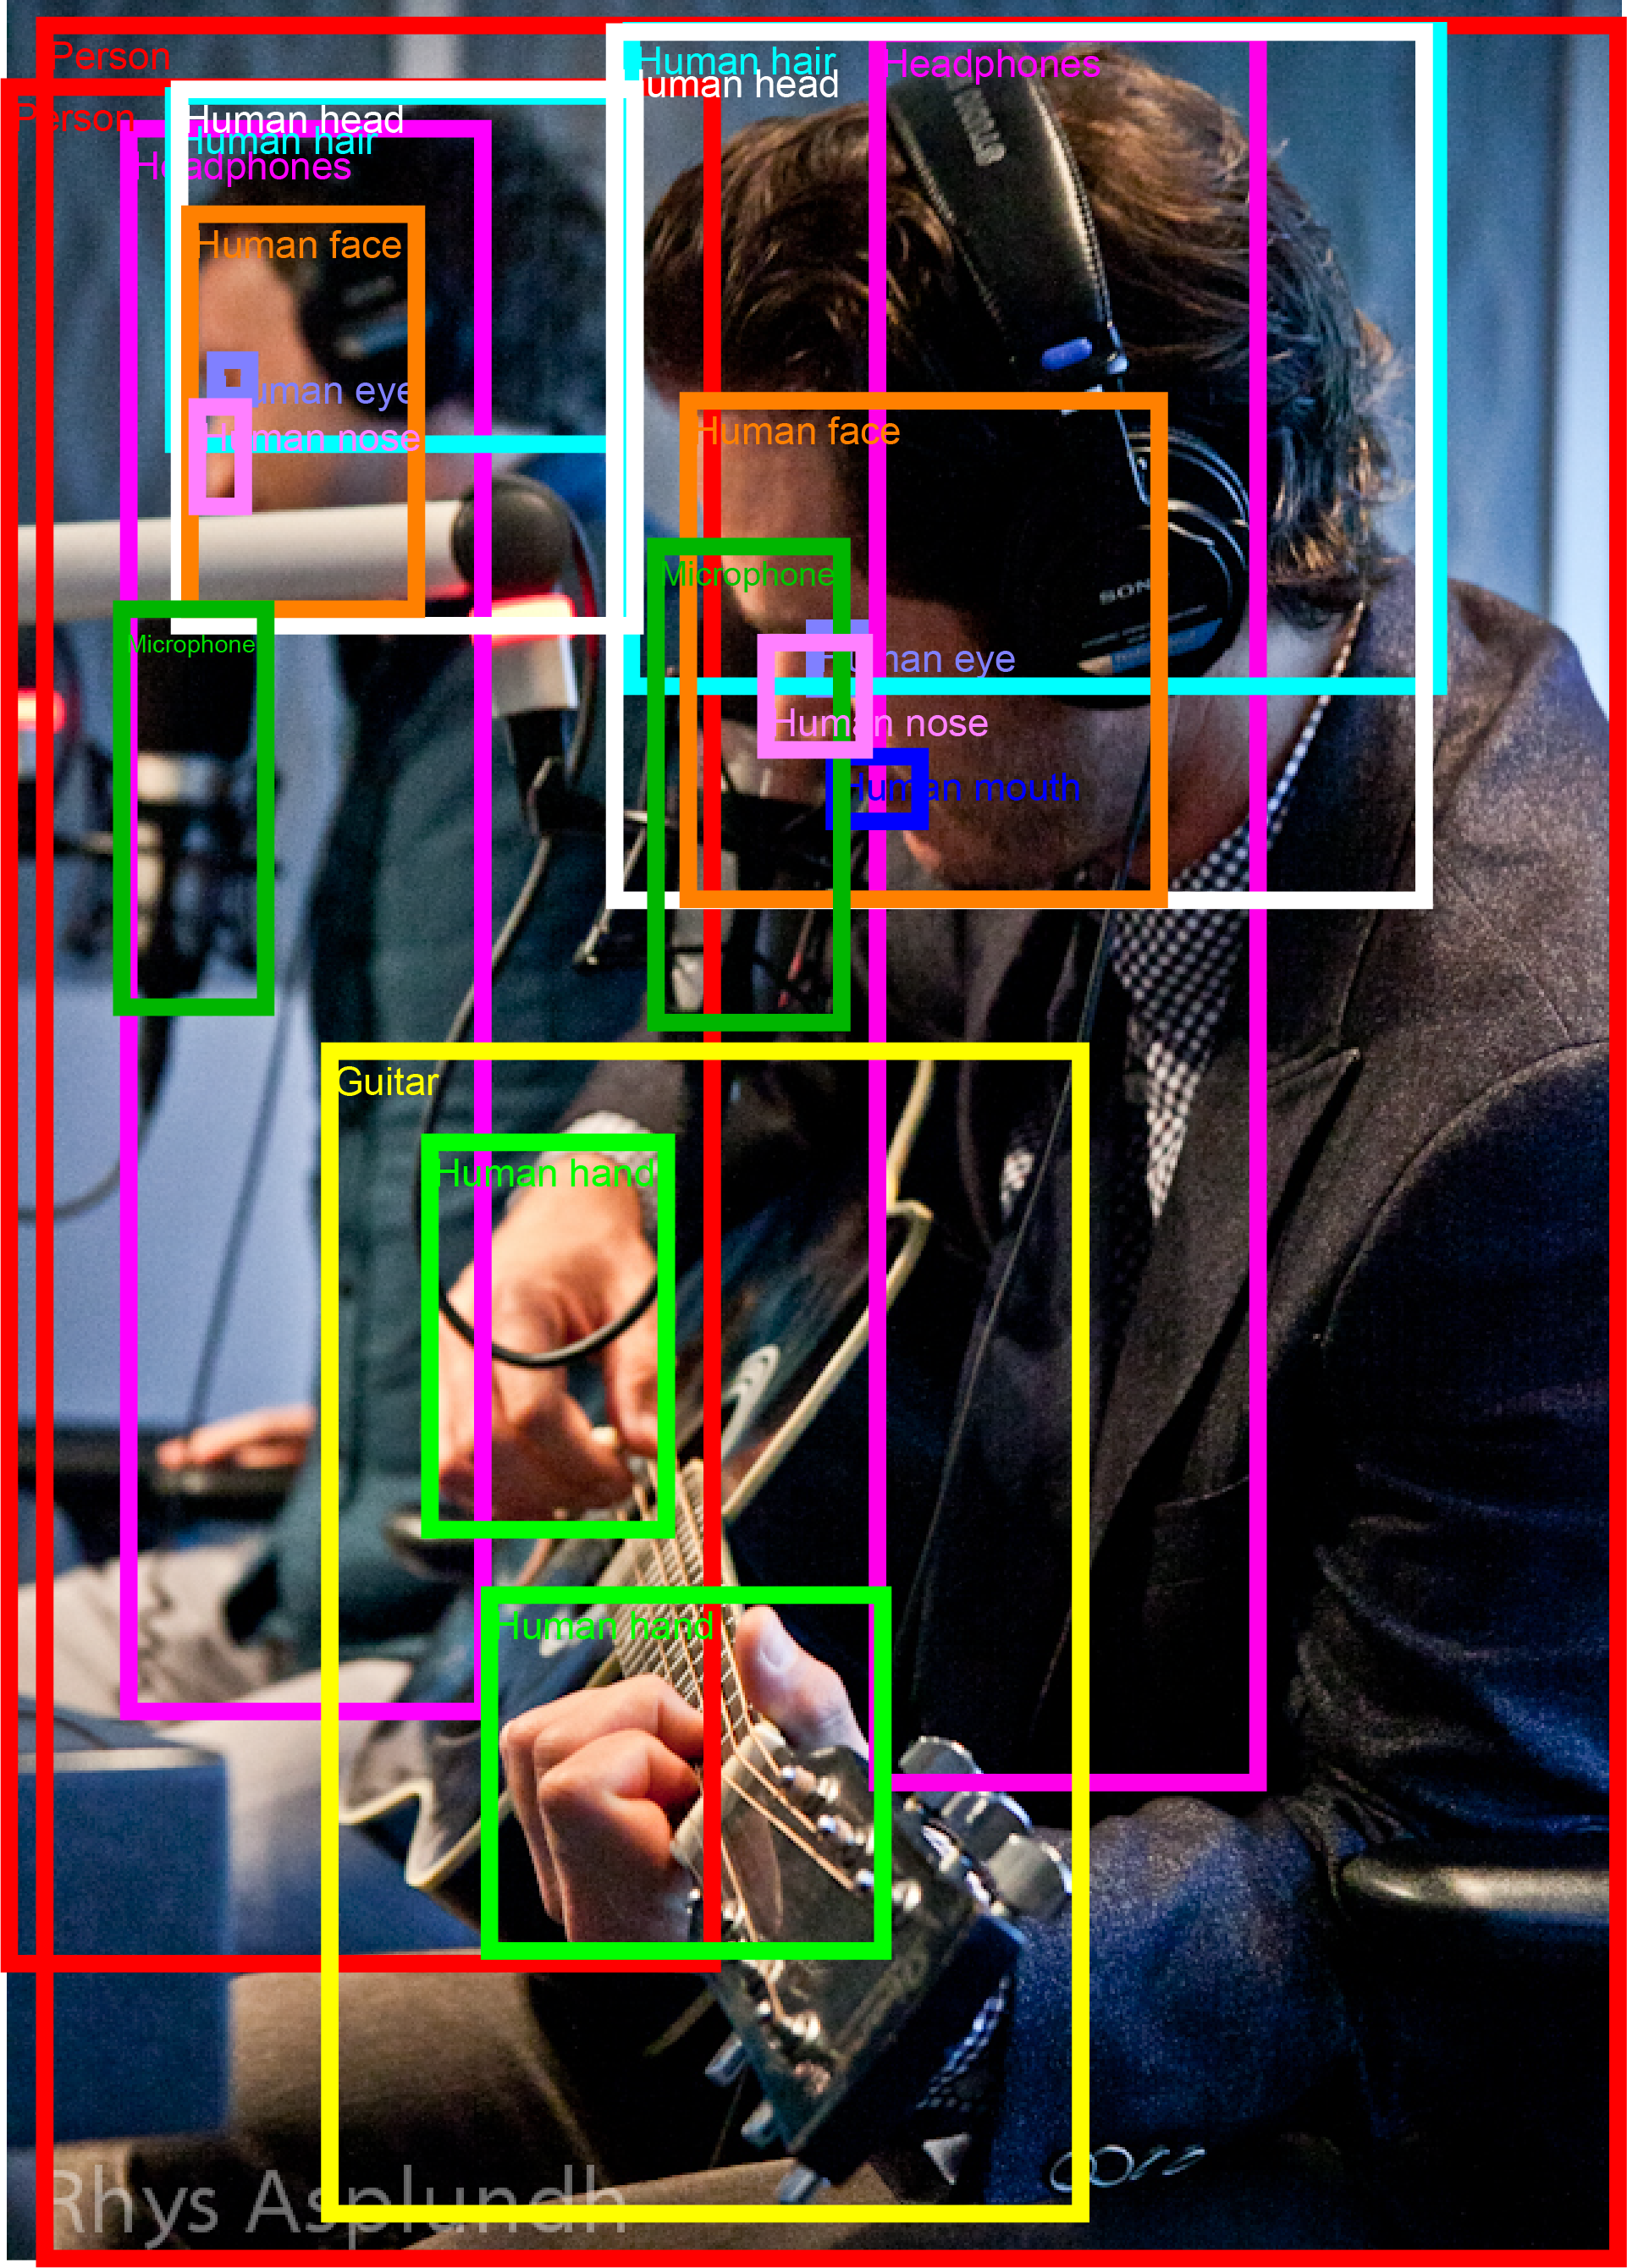
\includegraphics[width=.7\textwidth]{intro-1.png}
	\caption{\scriptsize Mark Paul Gosselaar plays the guitar by Rhys A. \cite{google:1}}
\end{figure}

The Kaggle challenge created by Google called Open Images 2019 - Object Detection \cite{kaggle} motivates this project. This Kaggle was created using the recent dataset announced, the Open Images Dataset v5 \cite{google:1}. This project proposes to show some strategies to solve the problem, giving a deep dive into some deep neural network architectures. 

\subsection{Problem Statement}

As described, the problem is going to be divided into two, the problem to create the correct bounding box and the problem to classify it. The idea is to create a simple pipeline with two models concatenated, and each model is going to optimize each technique.

The first model, called Bounding Box Identifier, is responsible for identifying all objects that could be classified by the Image Classifier Model. The loss function of this model is going to be the IoU (Intersection over Union) - described better in the next subsection.

On the other side, for the Image Classifier model, it is going to use the Categorial Crossentropy as a loss function.

\begin{figure}[ht]
	\centering
	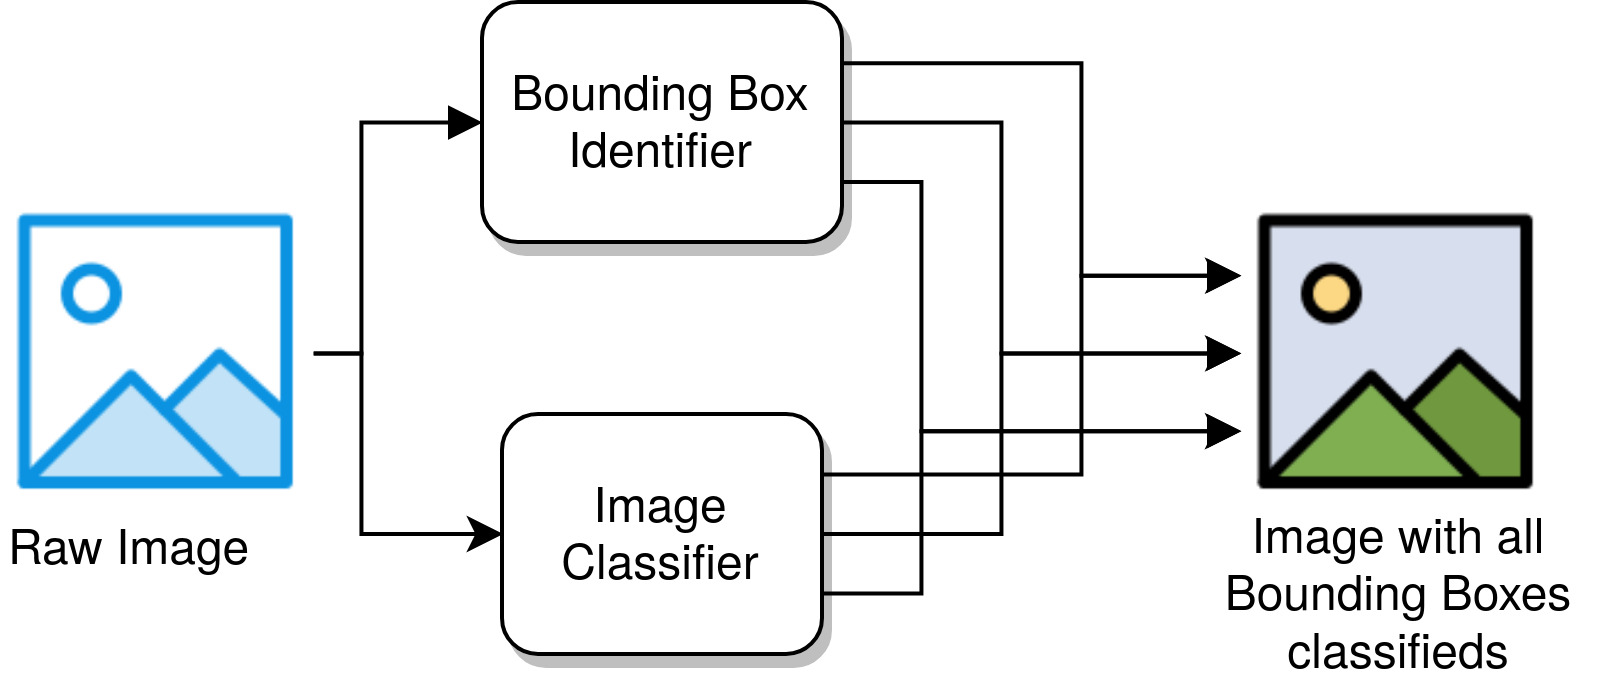
\includegraphics[width=1\textwidth]{high-level-architecture.jpg}
	\caption{\scriptsize High level Model Pipeline}
\end{figure}

It is import to explaining more about the loss functions. 

The Categorical Crossentropy used in the Classifier model is straightforward since it is a multiclass classifier. The idea is to compare for each class each distribution of the predictions made with the labeled distribution.

The IoU metric used as loss function arrives because mAP derives directly from the IoU. Since the mAP is going to be used as a metric to compare all models, it sounds reasonable to use IoU as a loss function to be optimized in the model responsible for creating the Bounding Boxes.

In the first step, the project starts to use the Transfer Learning technique in many famous networks - such as ResNet-N layers \cite{resnet}, Inception-V4 \cite{inception}, Xception \cite{xception}, and Inception-ResNets \cite{inception} - for both models, Object Identification, and Classifier. With Transfer Learning, we expect to achieve some reasonable results.

For the second and final step of the project, this work proposes to create, at minimum, one new architecture that could face other architectures seen above.

\subsection{Metrics}

The metric proposed by Google in the competition is the mean Average Precision (mAP) \cite{map}, a very didactic explanation about the metric could be found in here \cite{medium:1} and \cite{medium:2}.

The mAP metric could be defined as

{\centering
	\begin{equation*}
	mAP = \frac{\sum\limits_{c=1}^{C}AP_c} {C}
	\end{equation*}}

where $C$ value is the number of all categories (classes).

To understand $AP_c$, it must comprehend first what is $IoU$. $IoU$ is the Intersection over Union. It is equal to the ratio of the $Area\ of\ Overlap$ and the $Area\ of\ Union$, considering the Predict bounding box (created by the model) and the Ground-truth bounding box (previously annotated).


\begin{figure}[!ht]
	\centering
	\subfloat[\scriptsize  Difference between a Predict bounding box with a Ground-truth bouding box \cite{pyimage}]{{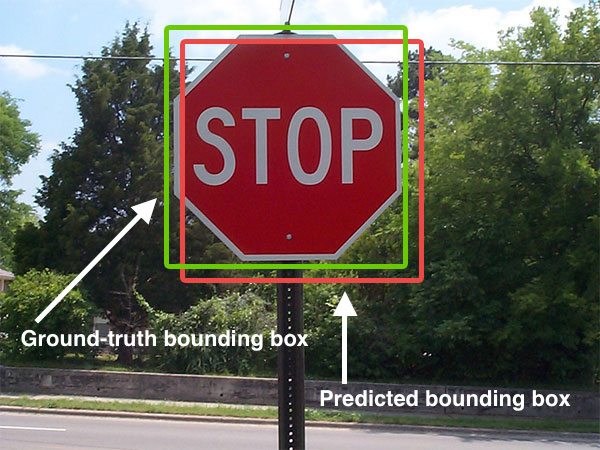
\includegraphics[width=5cm]{iou_stop_sign} }}%
	\qquad
	\subfloat[\scriptsize IoU visual represented \cite{pyimage}]{{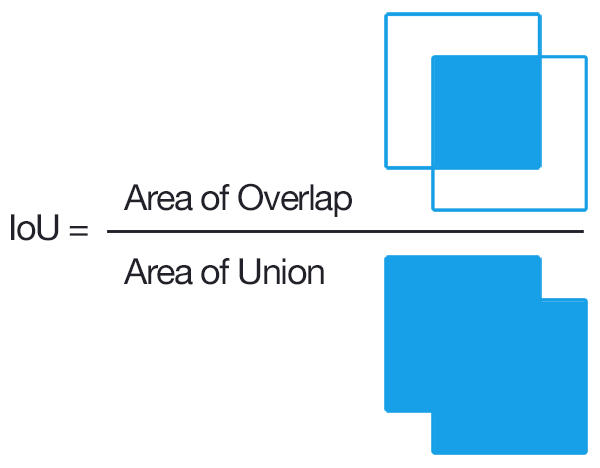
\includegraphics[width=5cm]{iou_equation} }}%
	%\caption{2 Figures side by side}%
	\label{fig:example}%
\end{figure}

Here, it is going to define:
\begin{align*}
TruePositive\ \dot=&\ IoU > 0.5 \\
FalsePositive\ \dot=&\ IoU < 0.5 \\
&or\ Duplicated PredictBoundingBox \\
FalseNegative\ \dot=&\ IoU > 0.5\ \\ 
&and \ WrongClassification
\end{align*}

With the concept of True Positive (TP), True Negatives (TN), and False Positives (FN) defined, it is possible to create a Precision-Recall Curve, which defines a function that gives a precision based on the recall.

\begin{figure}[!ht]
	
	\centering
	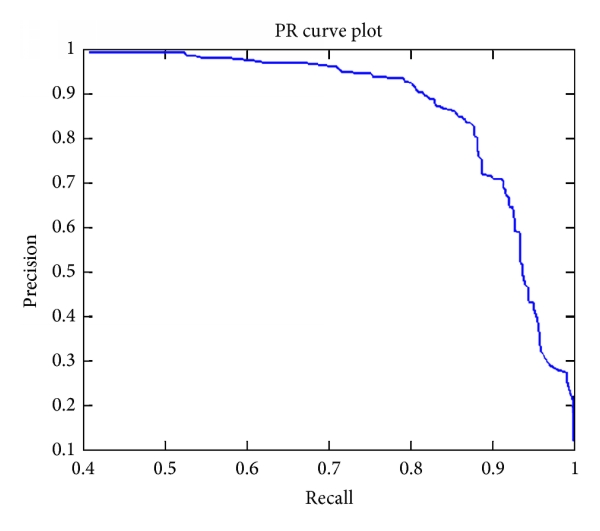
\includegraphics[width=.5\textwidth]{precision-recall.png}
	\caption{\scriptsize Precision-Recall curve \cite{medium:1}}
	
\end{figure}

So by definition, $AP_c$ (Average Precision of some category c), is defined as an Area Under the Curve ($AUC$) of the Precision-Recall curve.

{\centering
	\begin{equation*}
	AP_c = \int_{0}^{1} p(r) dr
	\end{equation*}
	where $p(r)$ is the precision defined in function of recall.}

It is essential to retain that in this project it is going to be used $AP_{50}$ (which uses a threshold of 0.5 in $IoU$ to define $TP$), but other average precision metrics could be used, like, $AP_{75}$ (with $IoU$ threshold of 0.75) or $AP_{90}$ (with $IoU$ threshold of 0.90).

\section{Analysis}

For the problem itself, there are two datasets (Image-level and bounding boxes), plus two files that describe each class used in the labeling process, and the relation among them.

About the classes, there are 600 unique classes, and they are represented as a graph. So they have inheritances. All classes start from a class that I called "Entity" (it has no name, in fact), and all other classes derive from it or from the classes that derive from it on some level. \hyperref[sec:appendix-a]{In the appendix A}, I expose all connections at each level (the deepest level is five).

The Train, Cross-Validation and Test set are already given by google. This project pretends to use the same distribution given. However, during the analysis it was possible to notice that there are some classes presented in Train set that are not presented in Test and Cross-Validation sets. The following table shows how much unique classes are present in each data set.

\begin{table}[ht]
	\footnotesize
	\centering
	\caption{ \footnotesize Unique classes in each Dataset and amount of Bounding Boxes }
	\label{table1}
	\begin{tabular}{lll}
		& Unique Classes & Count of Boubing Boxes \\
		\rowcolor[HTML]{EFEFEF} 
		Train            & 599            & 14,609,671             \\
		Cross-Validation & 570            & 303,980                \\
		\rowcolor[HTML]{EFEFEF} 
		Test             & 583            & 937,327               
	\end{tabular}
\end{table}

Besides that, the distribution of each class is not uniform. 30 classes are responsible for 80\% of bounding boxes labels, and 300 classes are responsible for less than 1\% of bounding boxes. Of course, this affects how the final model performs in a random image.

\begin{figure}[!ht]
	\centering
	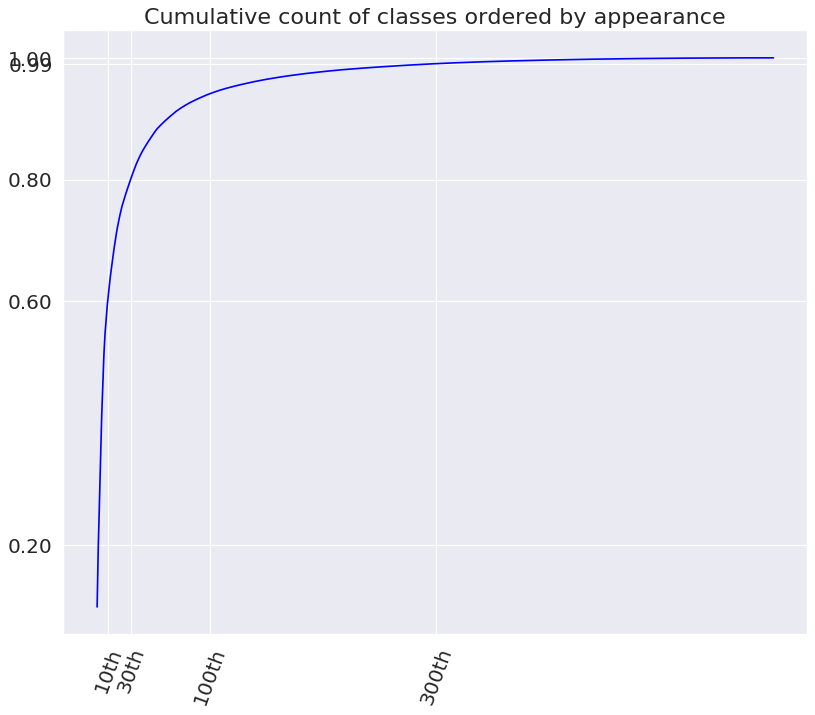
\includegraphics[width=0.7\textwidth]{cumulative-classes.png}
	\caption{\scriptsize Cumulative count of classes order by appearance}
\end{figure}

\begin{figure}[!ht]
	\centering
	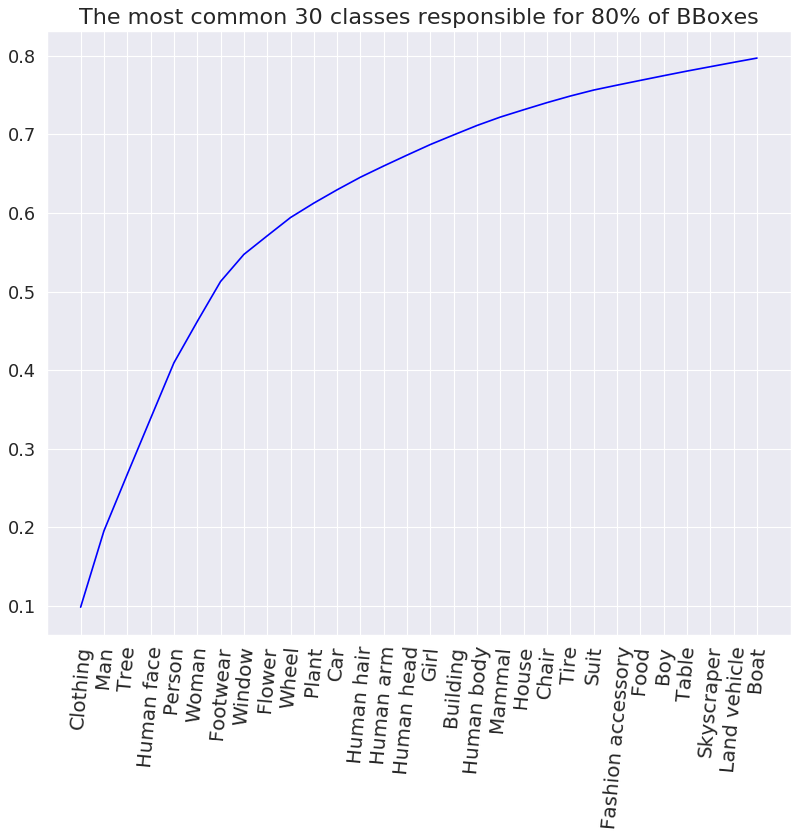
\includegraphics[width=0.7\textwidth]{30-most-frequently.png}
	\caption{\scriptsize The thirty classes with more appearance}
\end{figure}

There are two datasets, image-level label and bounding boxes, both divided by three (train, test, cross-validation). Google explains in the blog \cite{imgdataset} how they create the Image-level dataset and how, with it, they create the bounding boxes dataset. The label-image set was created, and a little part of it (around 1.7 million images) were chosen to have more granular work. The labels previously created were relabeled and transformed in bounding boxes that identify, not only what is the object, but the position of those objects. This work only uses the bounding boxes dataset.

About Bouding Box Dataset, some points must be concerned.
The labels in the original data set are encoded (probably to avoid mismatch and homonyms). In the analysis process they were converted to semantic labels (using an auxiliary dataset provided by google). However, in modeling, it is going to use the encoded version. 

\begin{table}[!ht]
	\footnotesize
	\centering
	\caption{ \footnotesize Amount of each flag in Bounding Box dataset }
	\label{table2}
	\begin{tabular}{llllll}
		& IsOccluded & IsTruncated & IsGroupOf & IsDepiction & IsInside \\
		\rowcolor[HTML]{EFEFEF} 
		Train            & 9,629,150  & 3,643,883   & 852,641   & 774,485     & 13,718   \\
		Cross-Validation & 134,497    & 69,698      & 26,360    & 14,181      & 2,200    \\
		\rowcolor[HTML]{EFEFEF} 
		Test             & 417,398    & 211,732     & 81,037    & 44,038      & 6,964   
	\end{tabular}
\end{table}

Beyond the label and the bounding boxes position, the dataset also has some flags (IsOccluded, IsTruncated, IsGroupOf, IsDepiction, IsInside). These flags are very helpful to debug the decisions that a model does.

"IsOccluded" points a Bounding Box that has a type of obstruction in it, making it more difficult to be understandable.

"IsTruncated" points a Bounding Box that ends or starts in some edges of the image.

"IsGroupOf" means that the label given is about a group of things, and the bounding box is around all of those things.

\begin{figure}[!ht]
	\centering
	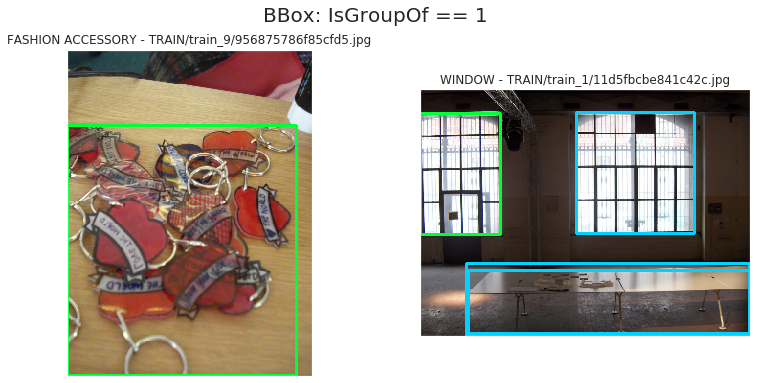
\includegraphics[width=1\textwidth]{isgroupof-true.png}
	\caption{\scriptsize Class Hierarchy - Second Level second part}
\end{figure}

\begin{figure}[!ht]
	\centering
	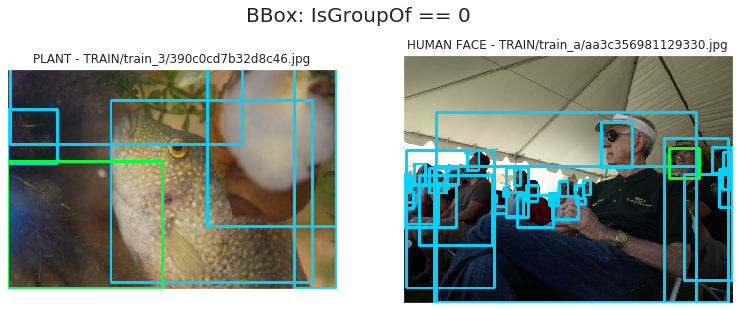
\includegraphics[width=1\textwidth]{isgroupof-false.png}
	\caption{\scriptsize Class Hierarchy - Second Level second part}
\end{figure}

"IsDepiction" represents bounding boxes that do not label the object itself, but a representation of the object. Draws, representation, costumes, are some examples.

"IsInside" is about the Bounding Boxes labeled inside rooms or buildings, with artificial light.

As stated, the distributions of classes are not uniform, and this is a big concern about how good the model will be. There is a more accurate and complete analysis, with a study of the correlations between flags and many other topics in all datasets. It can be checked in here \cite{eda}.


\subsection{Data Exploration}
\subsection{Exploratory Visualization}
\subsection{Algorithms and Techniques}
\subsection{Benchmark}
\section{Methodology}
\subsection{Data Preprocessing}
\subsection{Implementation}
\subsection{Refinement}
\section{Results}
\subsection{Model Evaluation and Validation}
\subsection{Justification}
\section{Conclusion}
\subsection{Free-Form Visualization}
\subsection{Reflection}
\subsection{Improvement}

\bibliographystyle{unsrt}
\bibliography{references.bib}{}

\begin{appendices}
	\section {Class hierarchy}
	\label{sec:appendix-a}
	
	\begin{figure}[!ht]
		\centering
		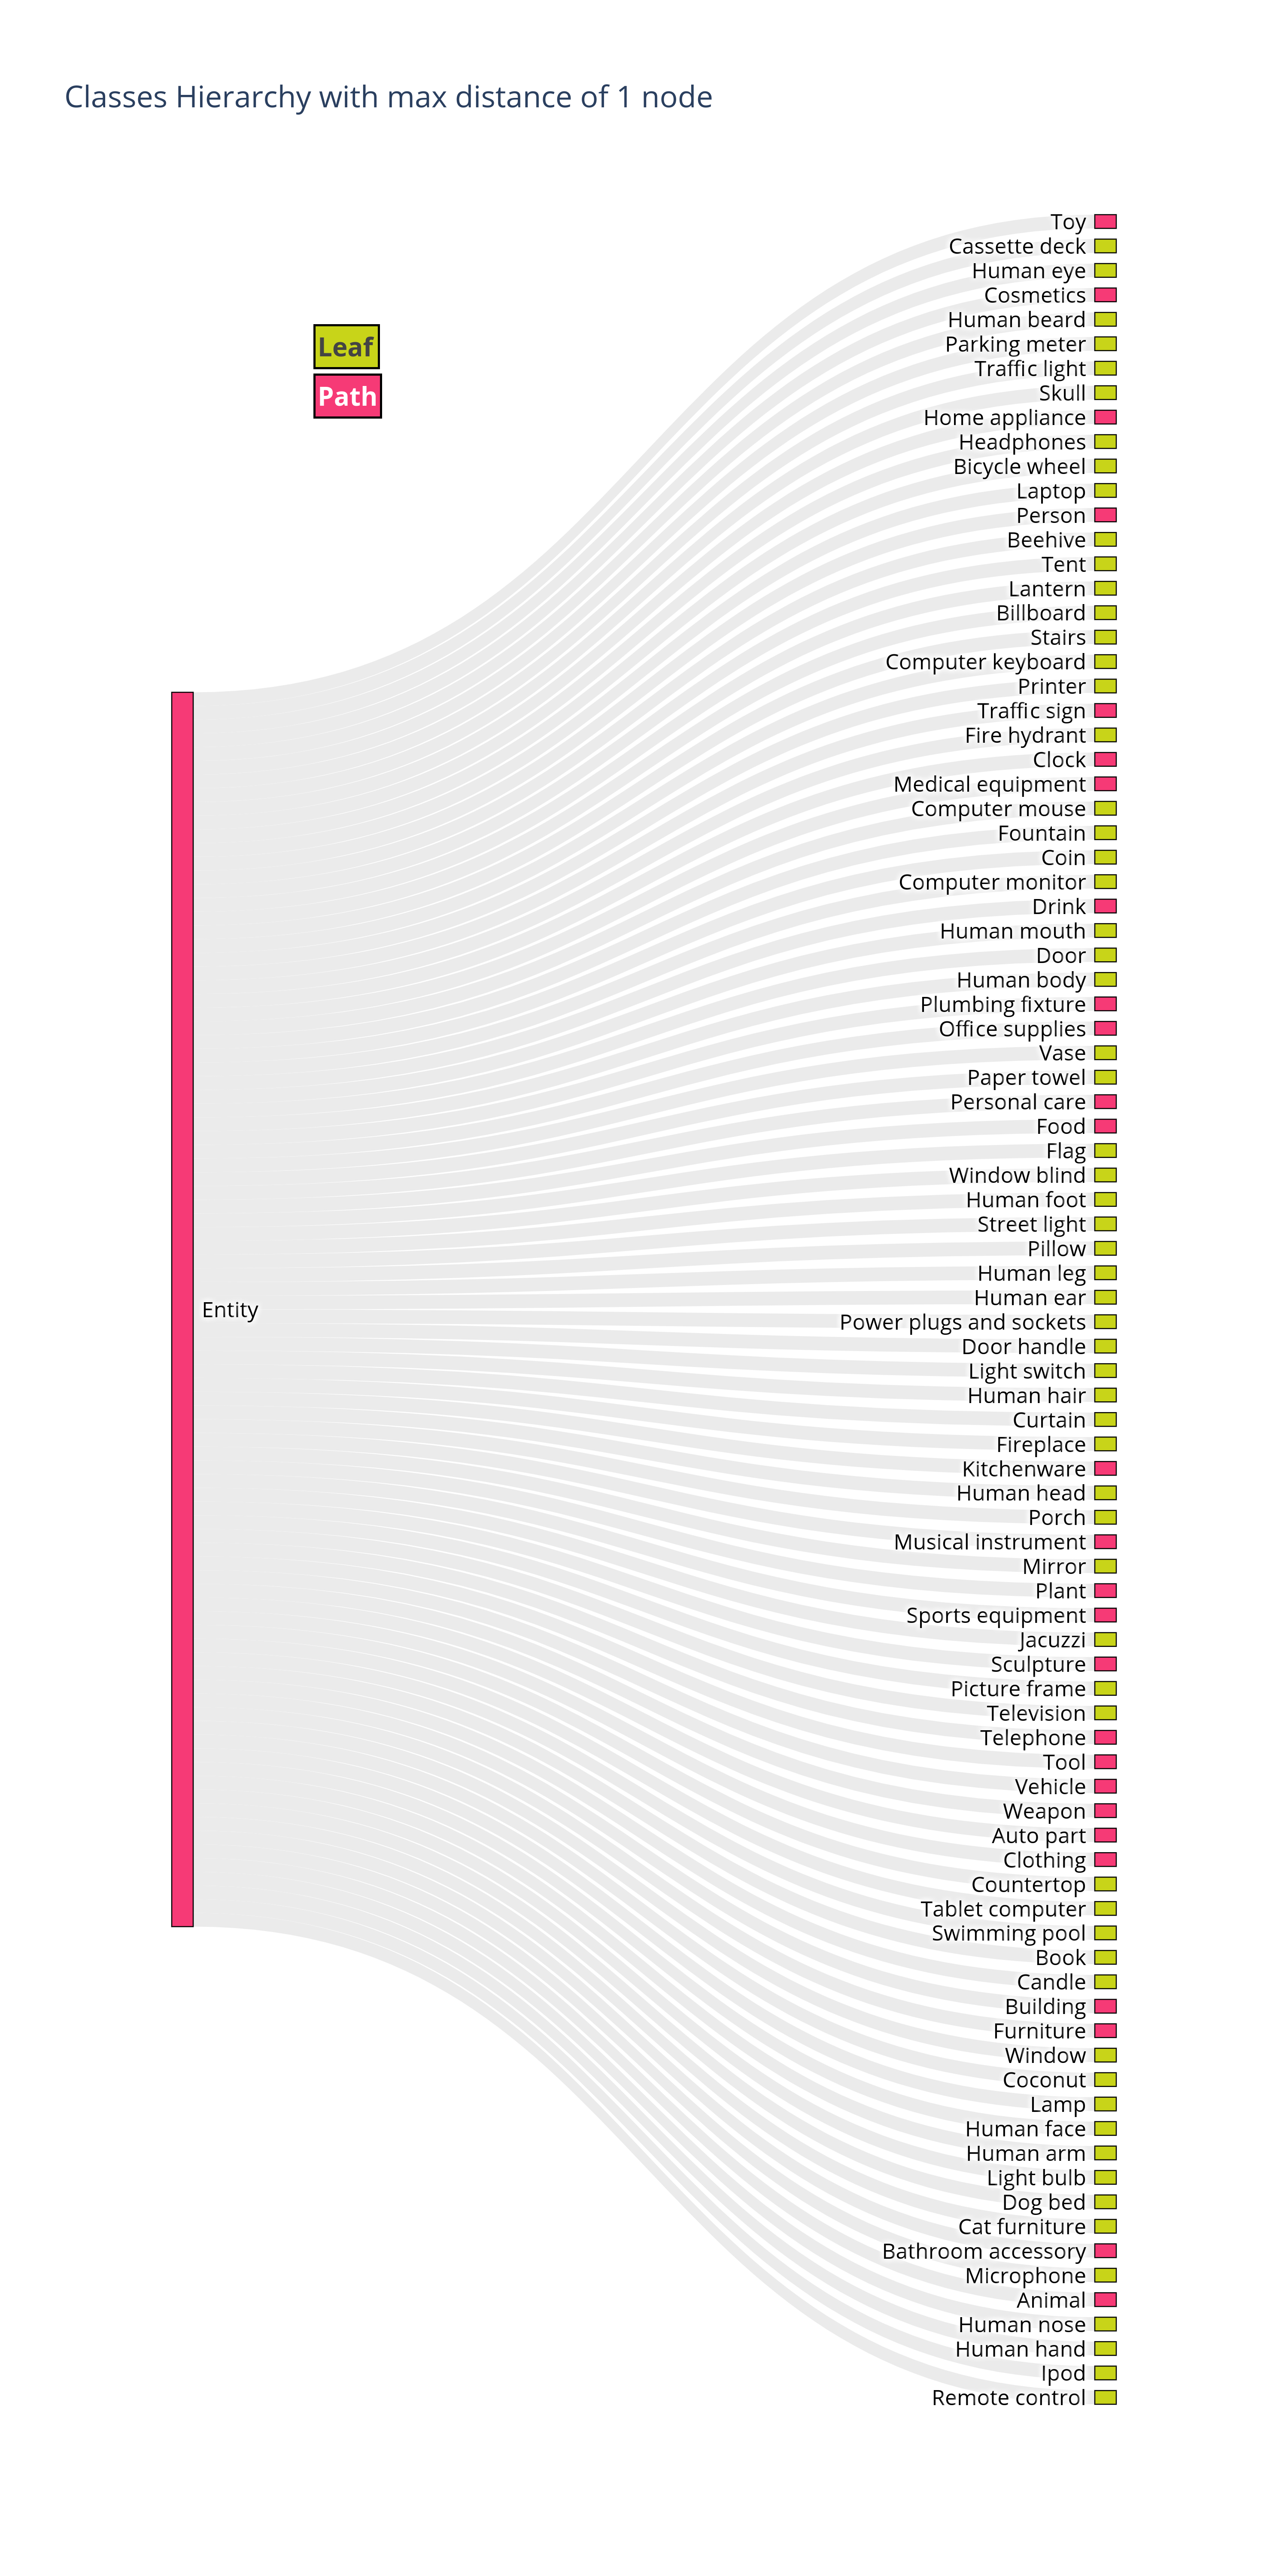
\includegraphics[width=0.7\textwidth]{lvl1_classes.png}
		\caption{\scriptsize Class Hierarchy - First Level}
	\end{figure}
	
	\begin{figure}[!ht]
		\centering
		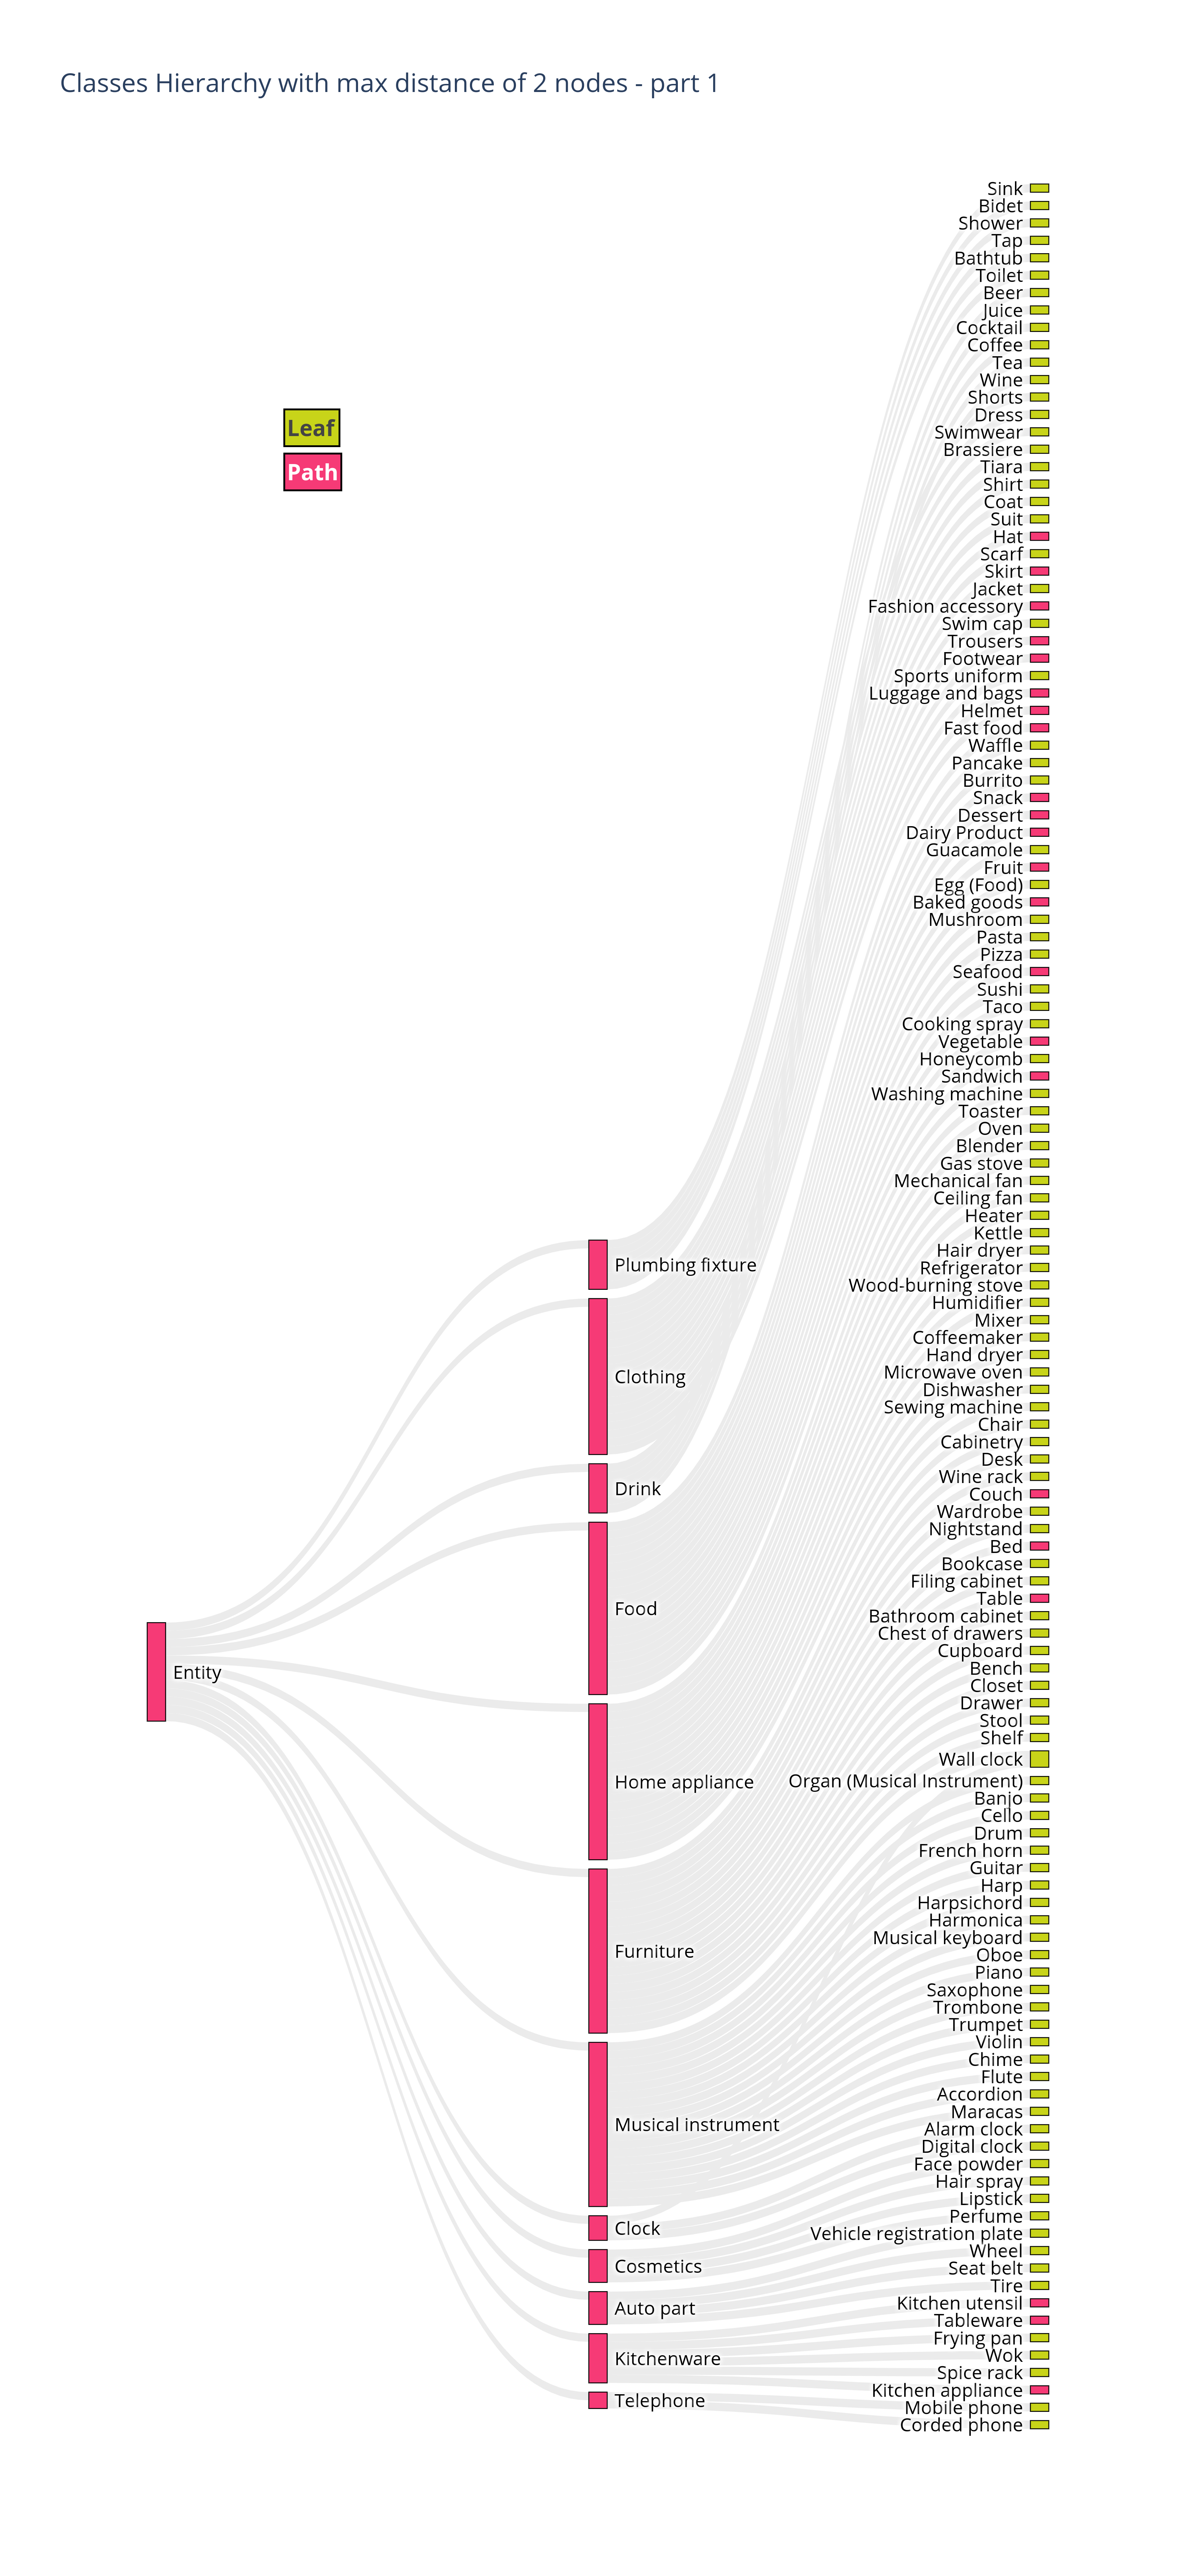
\includegraphics[width=0.8\textwidth]{lvl2_classes_pt1.png}
		\caption{\scriptsize Class Hierarchy - Second Level first part}
	\end{figure}
	\begin{figure}[!ht]
		\centering
		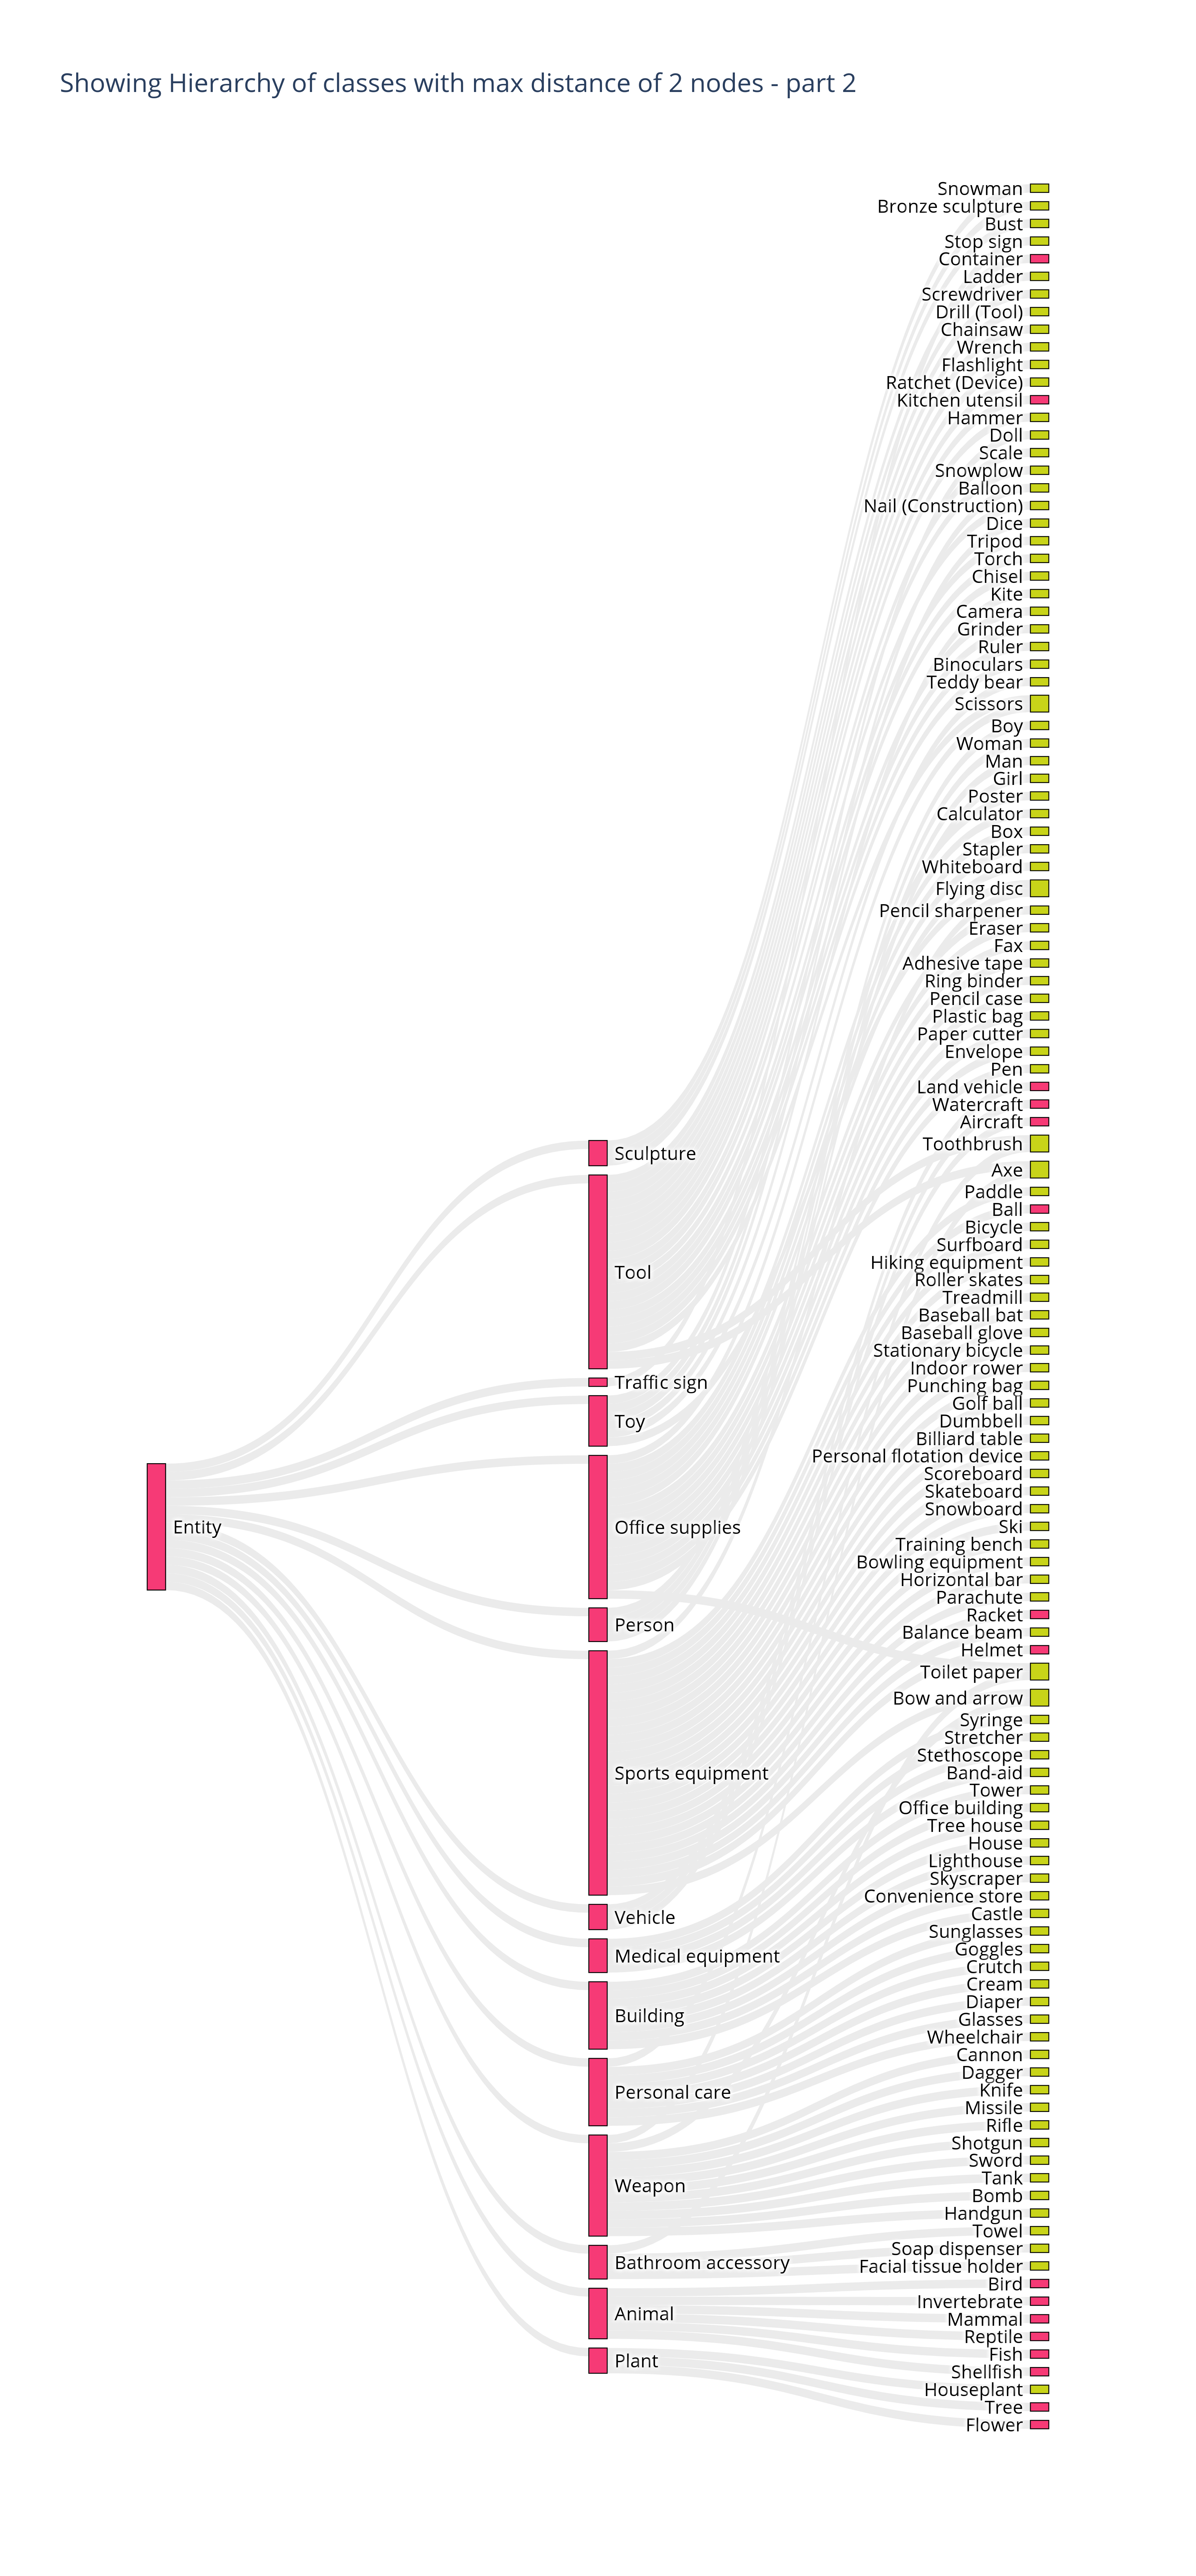
\includegraphics[width=0.8\textwidth]{lvl2_classes_pt2.png}
		\caption{\scriptsize Class Hierarchy - Second Level second part}
	\end{figure}
	
	\begin{figure}[!ht]
		\centering
		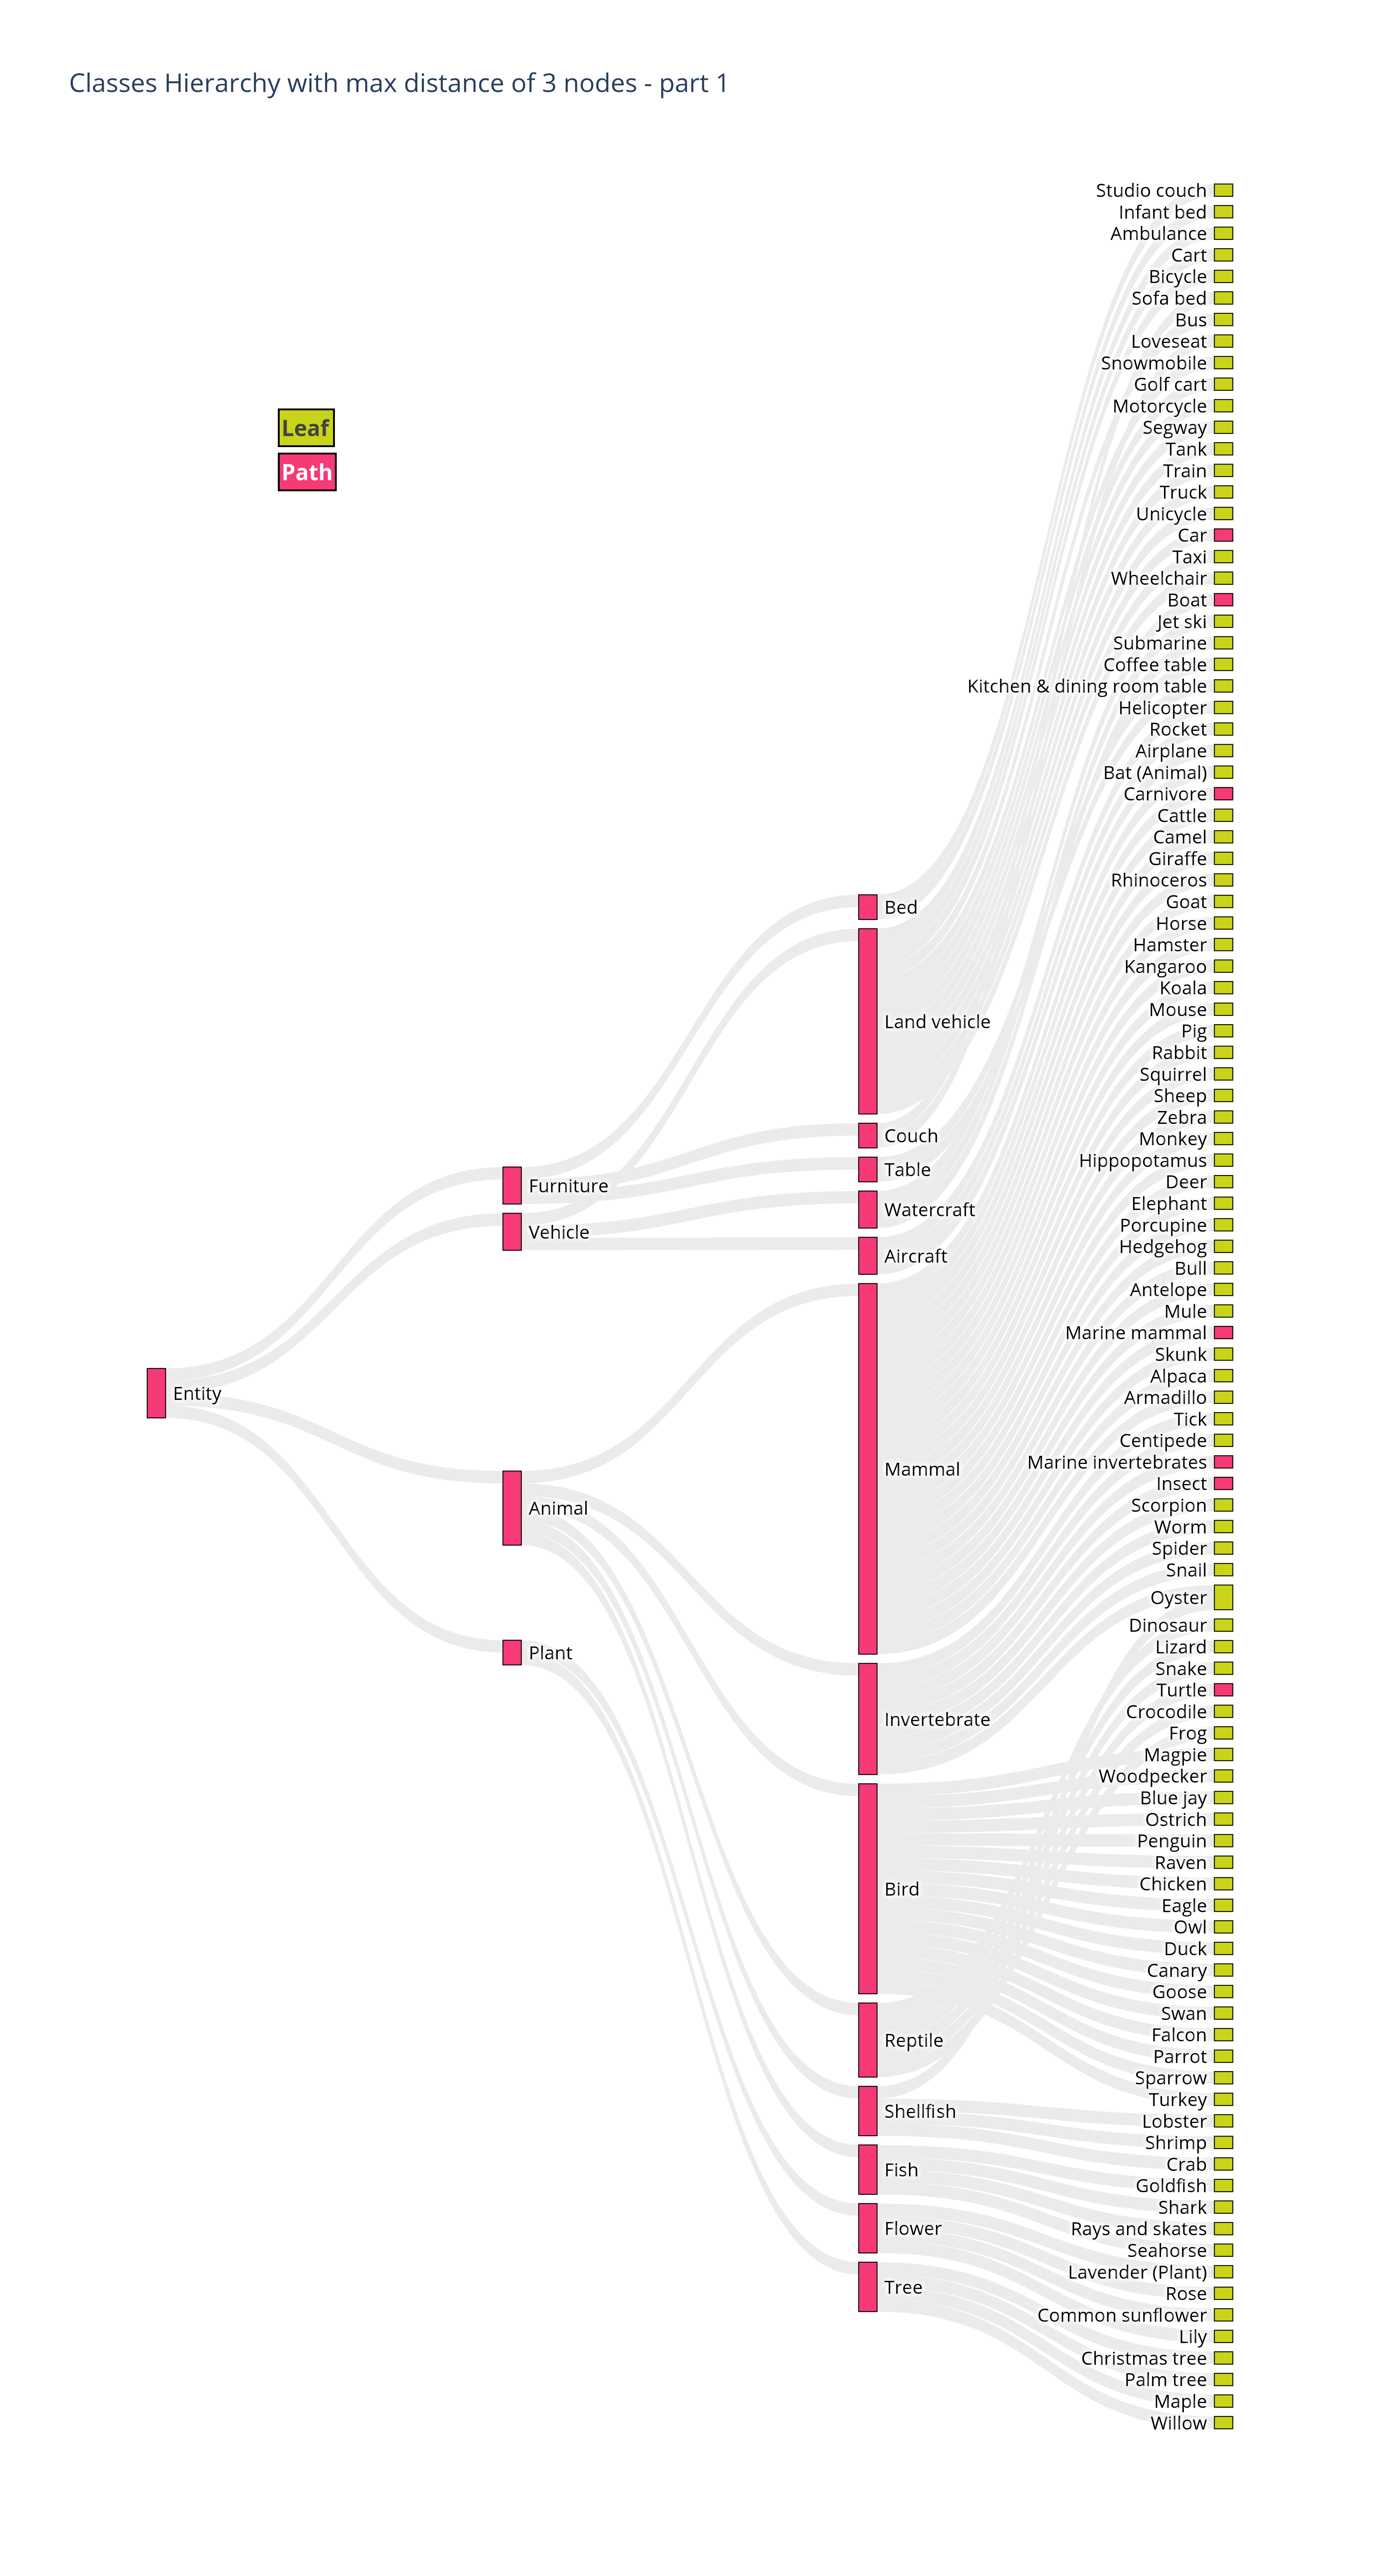
\includegraphics[width=0.8\textwidth]{lvl3_classes_pt1.png}
		\caption{\scriptsize Class Hierarchy - Third Level first part}
	\end{figure}
	\begin{figure}[!ht]
		\centering
		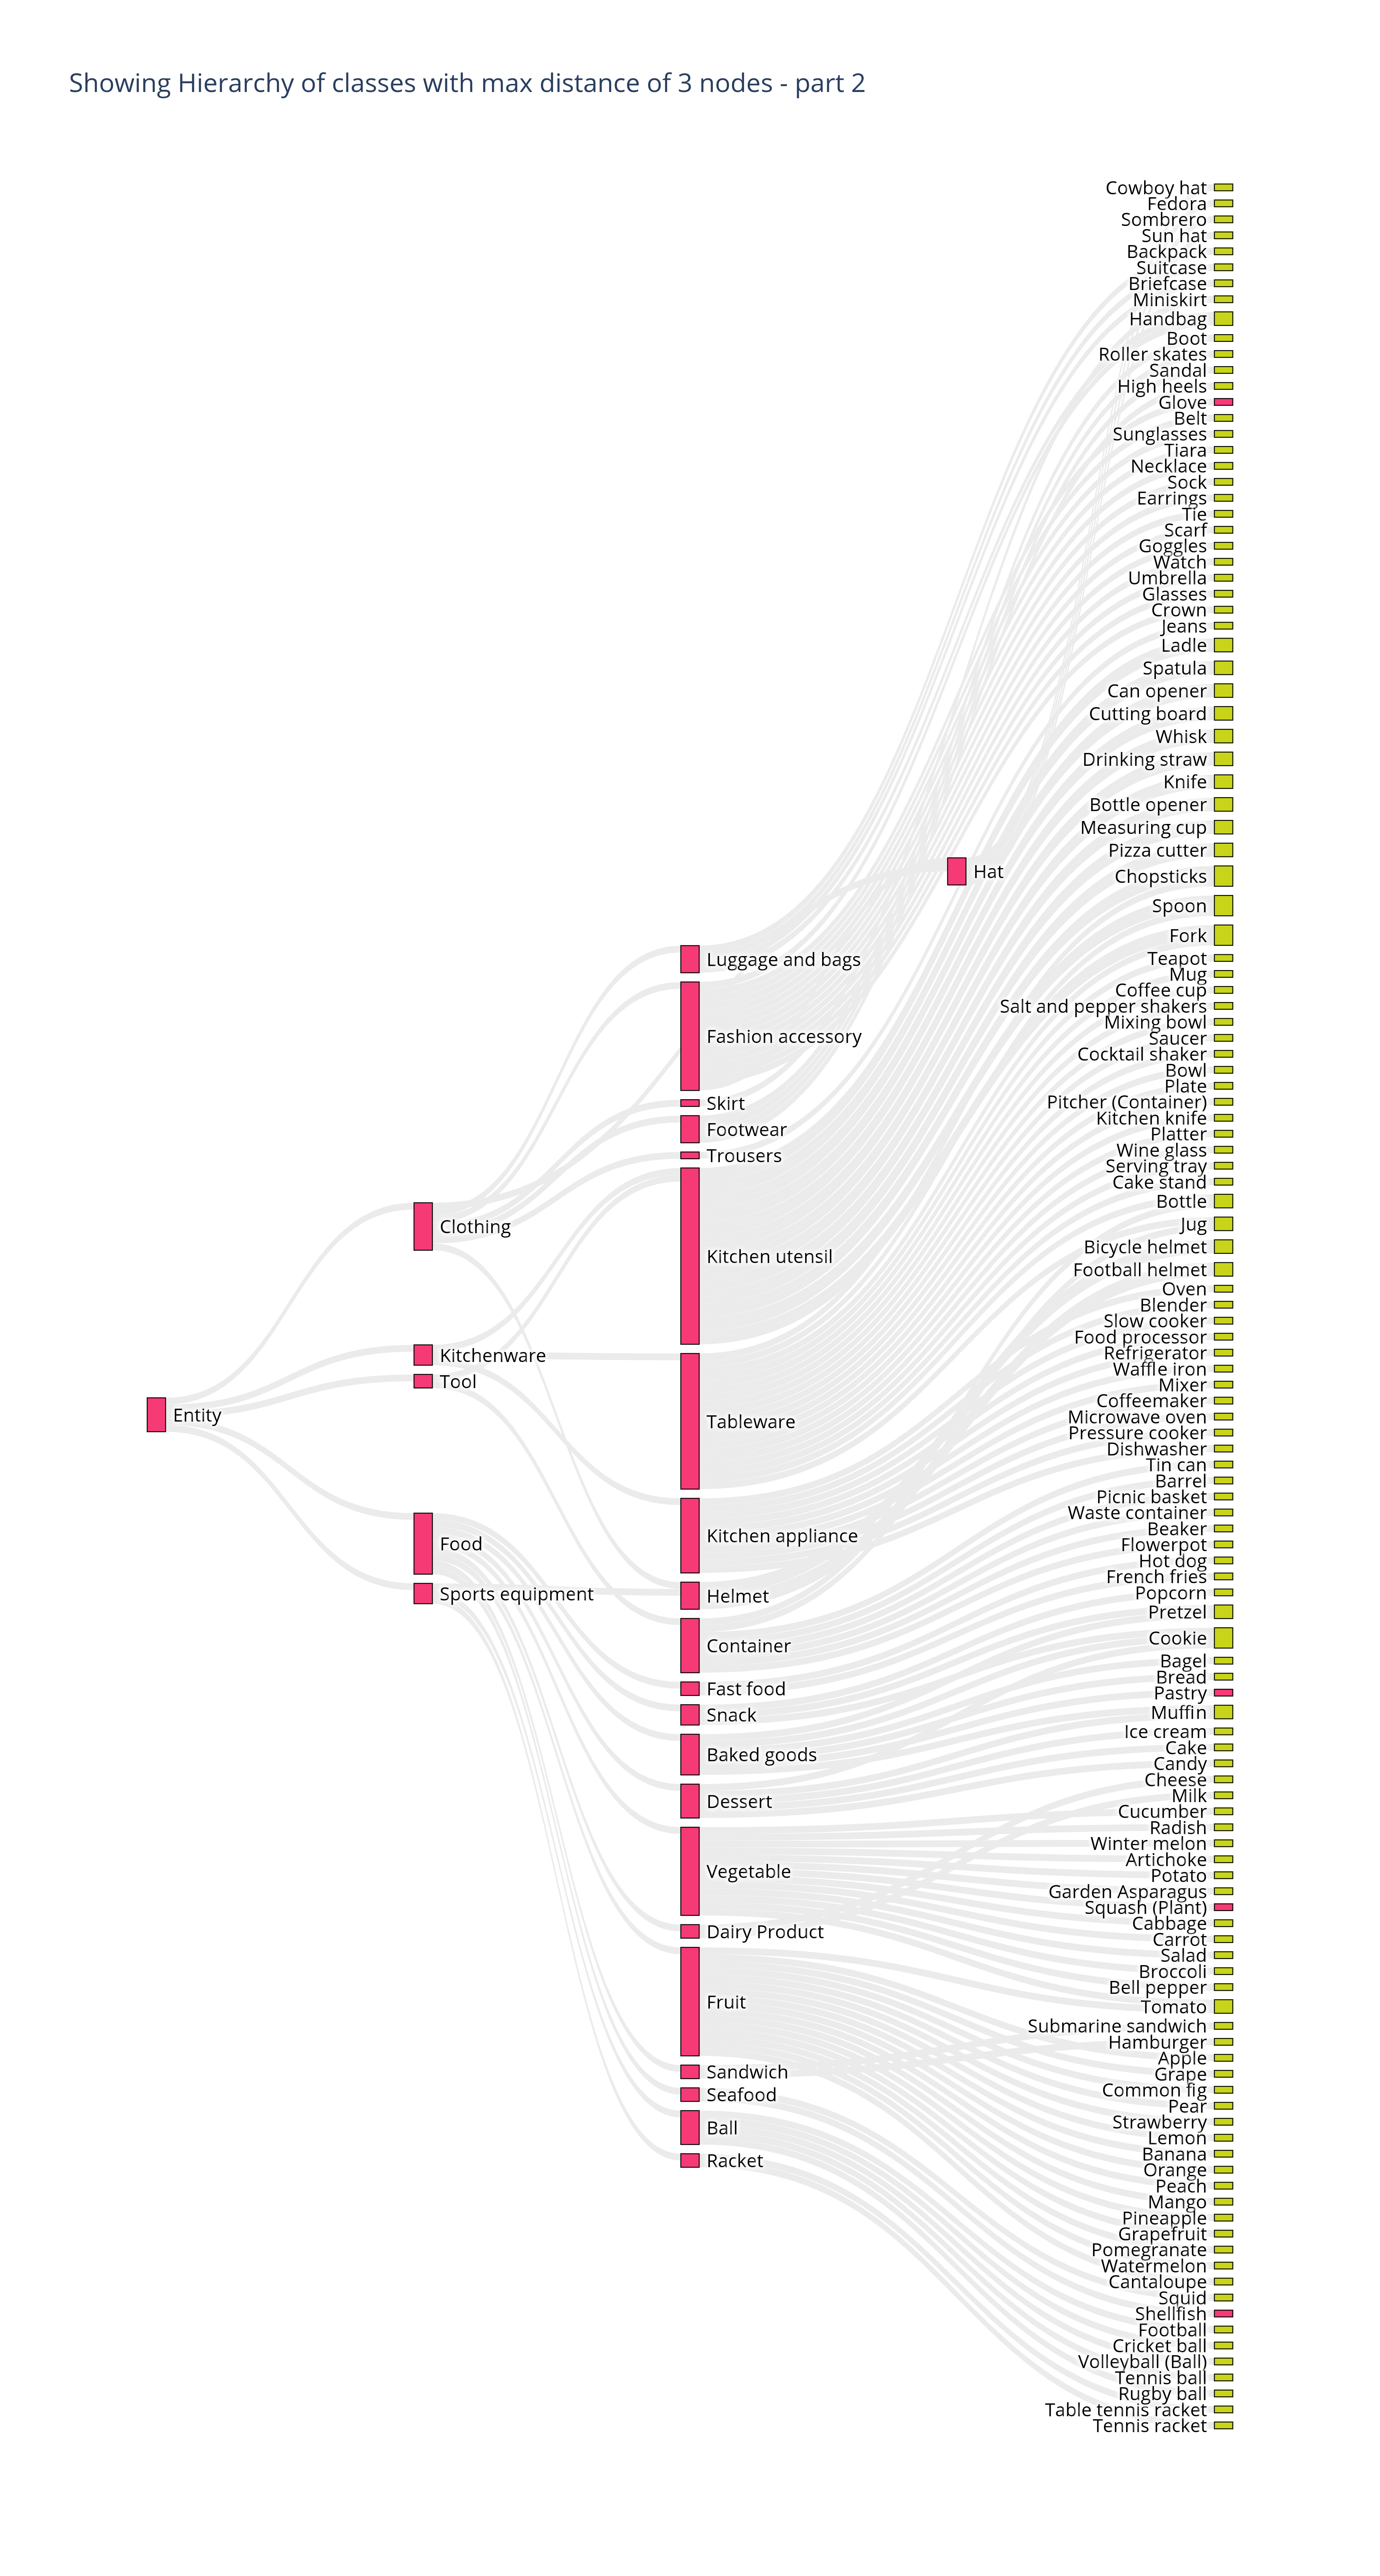
\includegraphics[width=0.8\textwidth]{lvl3_classes_pt2.png}
		\caption{\scriptsize Class Hierarchy - Third Level second part}
	\end{figure}
	
	\begin{figure}[!ht]
		\centering
		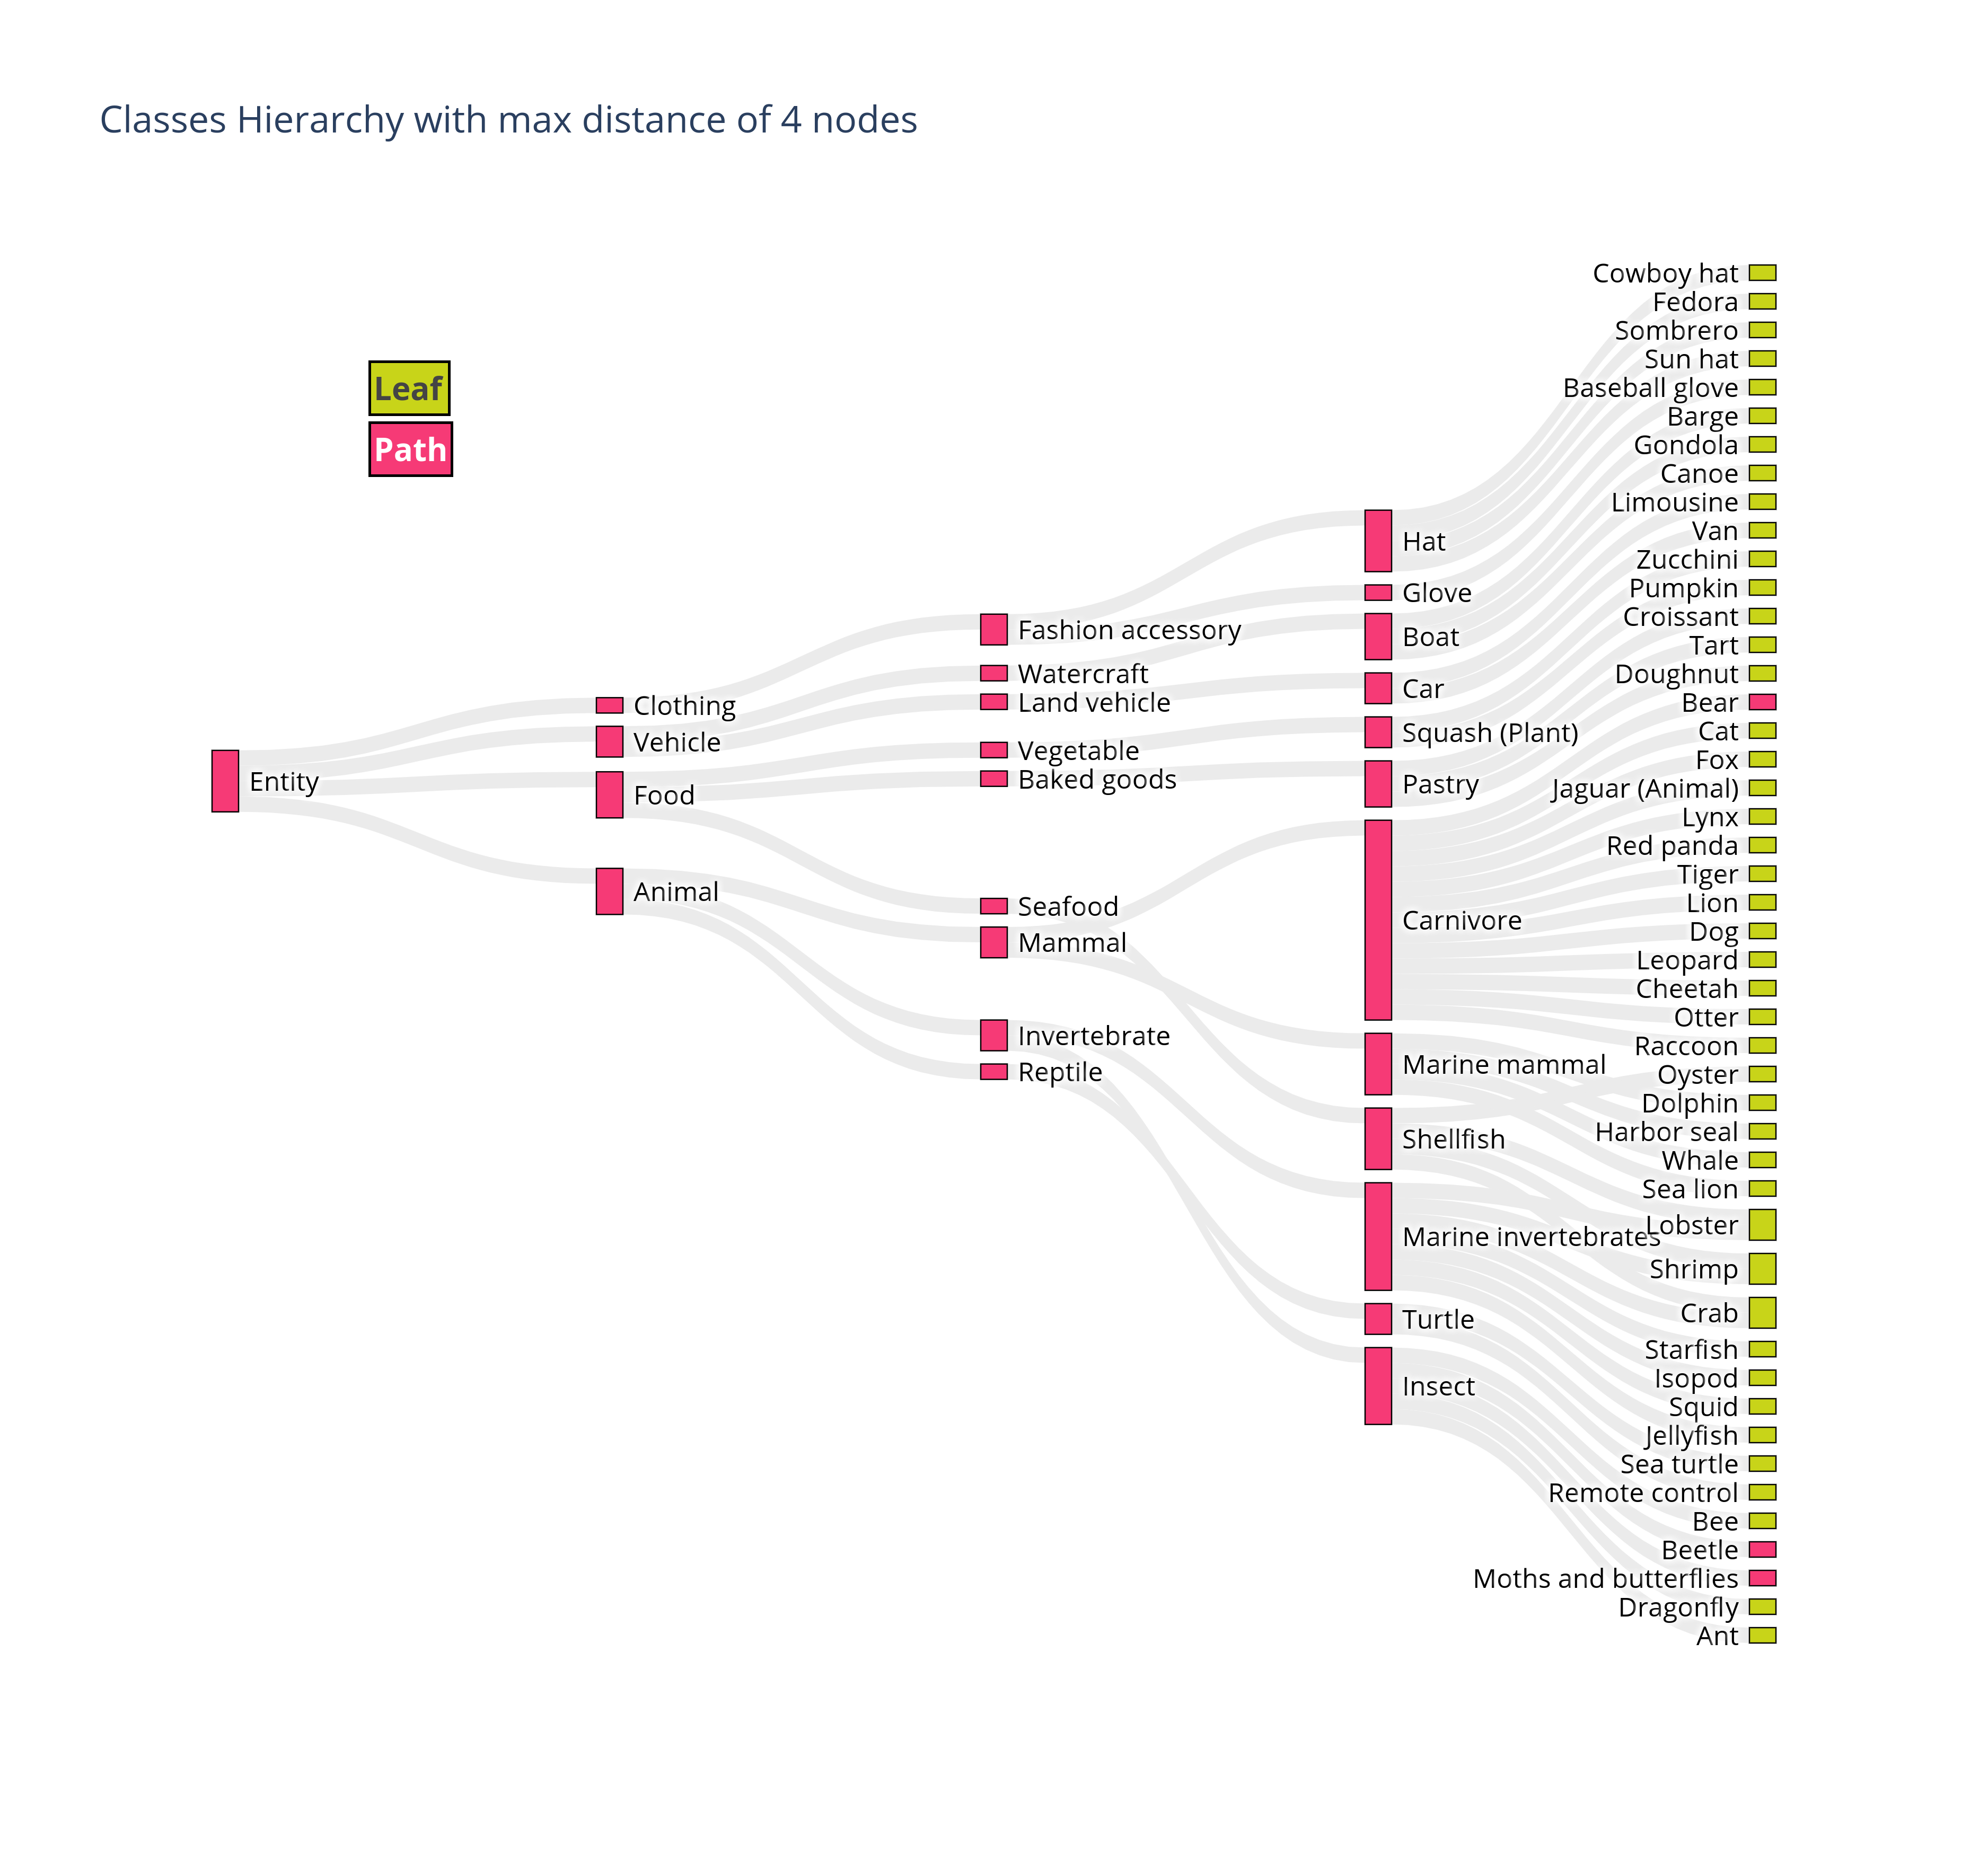
\includegraphics[width=0.8\textwidth]{lvl4_classes.png}
		\caption{\scriptsize Class Hierarchy - Fourth Level}
	\end{figure}
	
	\begin{figure}[!ht]
		\centering
		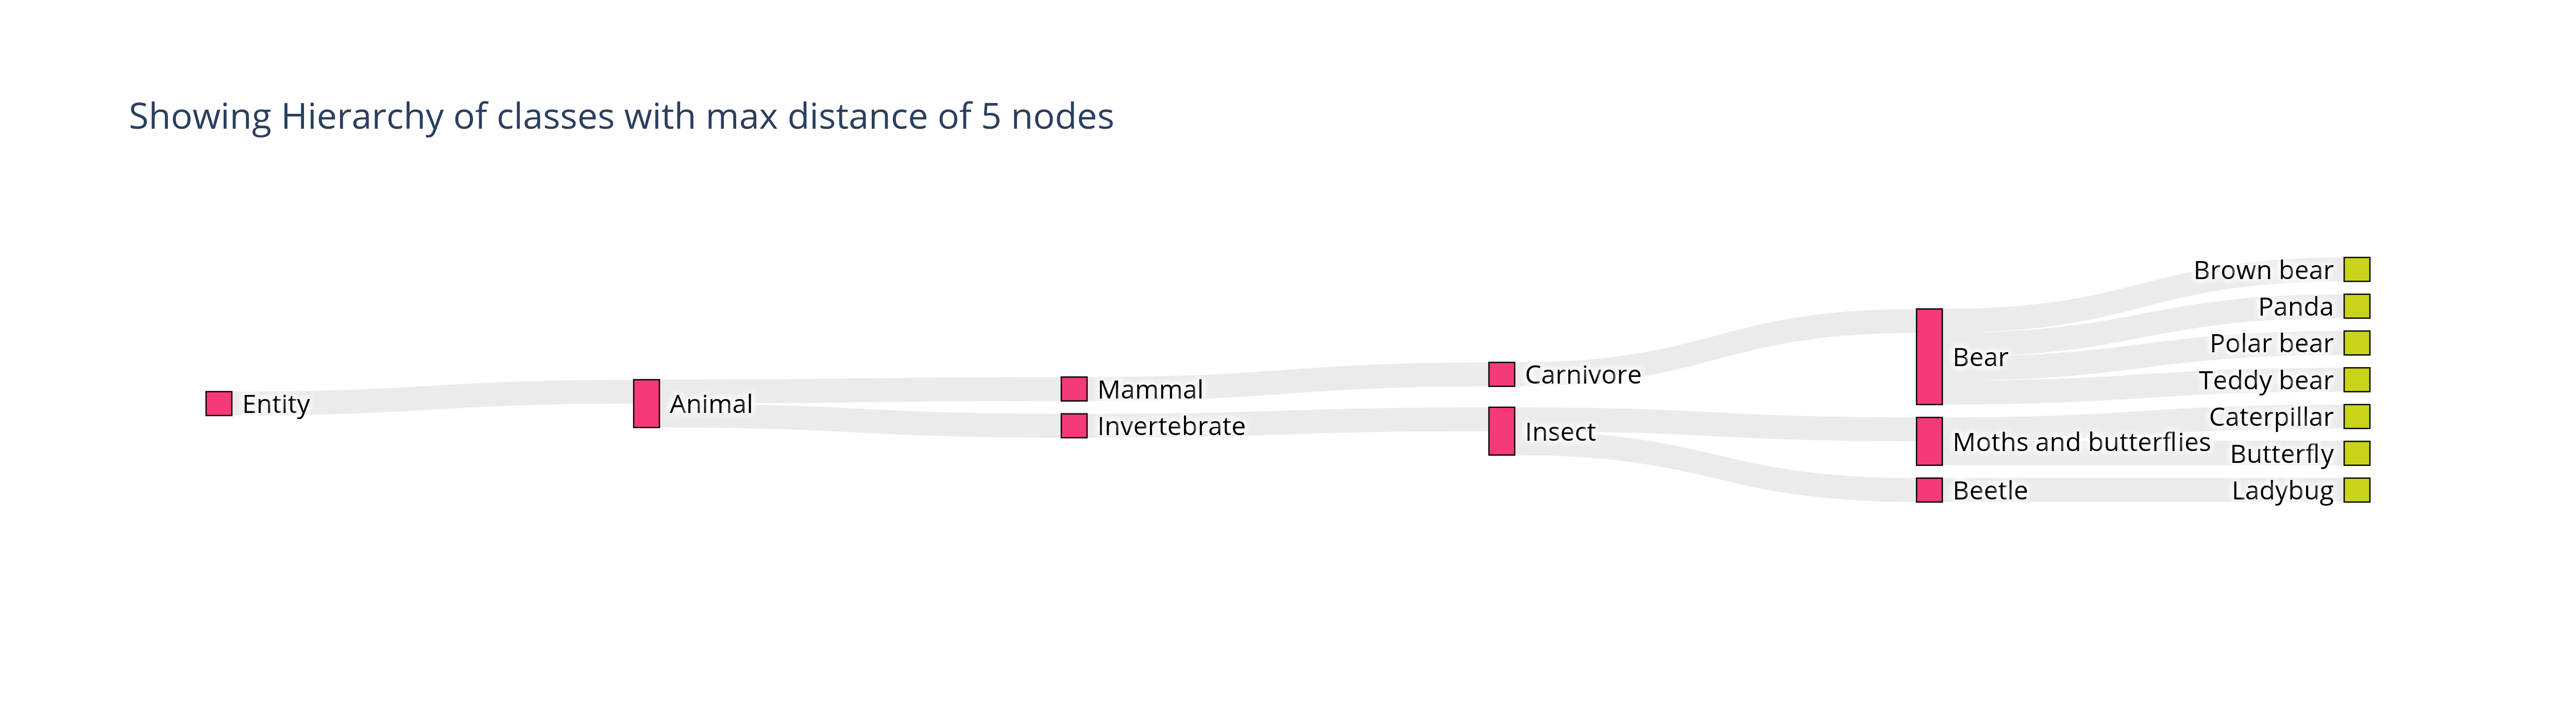
\includegraphics[width=0.8\textwidth]{lvl5_classes.png}
		\caption{\scriptsize Class Hierarchy - Fifth Level}
	\end{figure}

\end{appendices}

\end{document}